\chapter{Appendix D}
\setcounter{figure}{0}
\renewcommand{\thefigure}{D.\arabic{figure}}
\renewcommand{\thesection}{D.\arabic{section}}

\begin{figure}
    \centering
    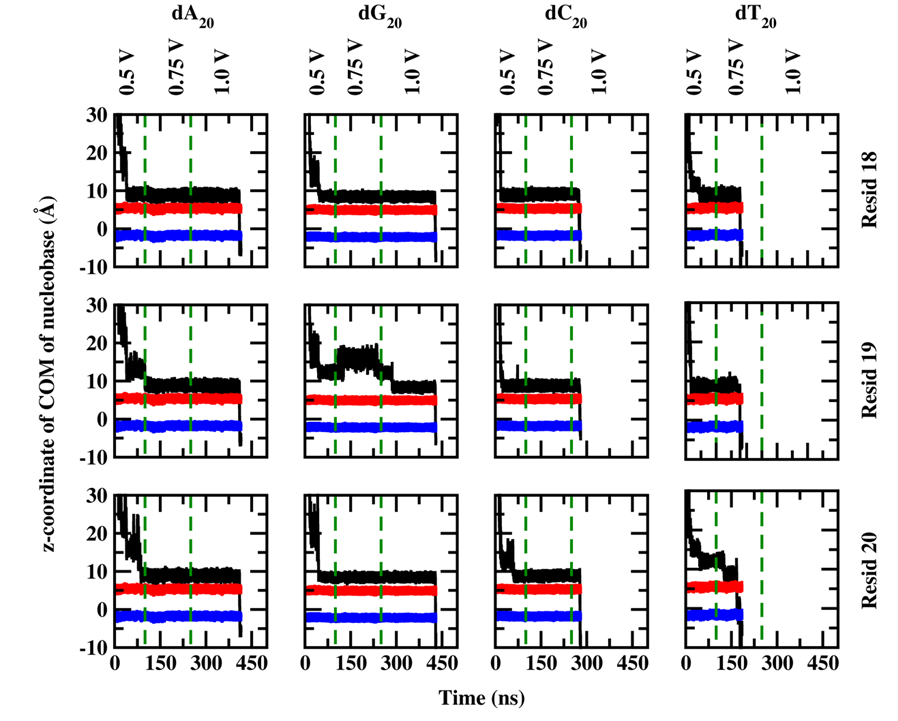
\includegraphics[width=\textwidth]{Appendix/Figures/D1_port.png}
    \caption[Time series plots for the z-coordinate of the center-of-mass of nucleotides at the 3’-end of the ssDNA obtained from additive simulations]{Time series plots for the z-coordinate of the center-of-mass of nucleotides at the 3’-end of the ssDNA obtained from additive simulations. The z-coordinate of the top (red) and the bottom (blue) sheet are also presented to indicate the relative distance of the 3’-end nucleotides to the graphene sheet. Time-series have been plotted till complete translocation is observed, or for 500 ns in case of incomplete translocations. Variations in the applied external bias have also been indicated.}
\end{figure}

\begin{figure}
    \centering
    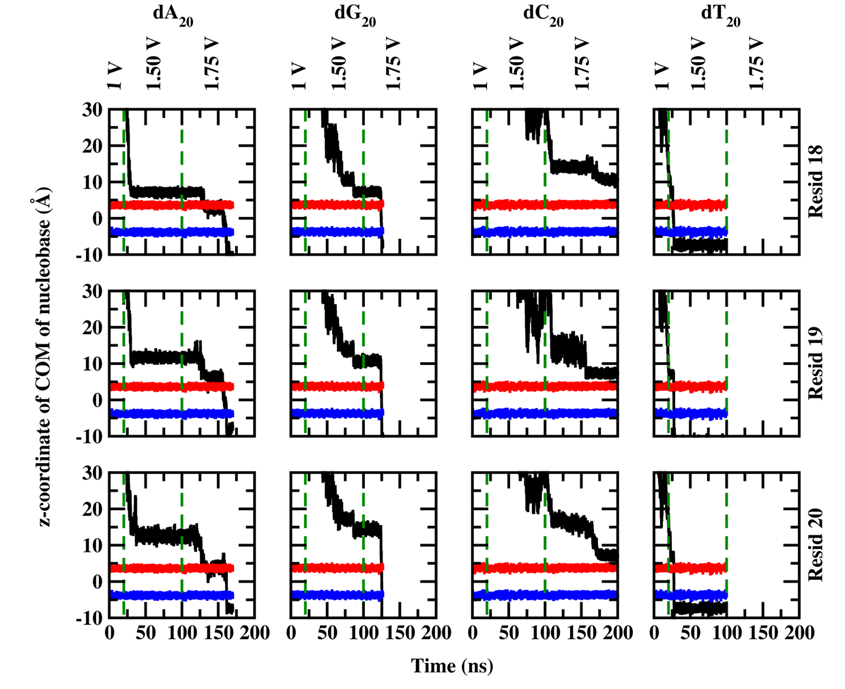
\includegraphics[width=\textwidth]{Appendix/Figures/D2_port.png}
    \caption[Time series plots for the z-coordinate of the center-of-mass of nucleotides at the 3’-end of the ssDNA obtained from Drude Polarizable FF simulations]{Time series plots for the z-coordinate of the center-of-mass of nucleotides at the 3’-end of the ssDNA obtained from Drude Polarizable FF simulations. The z-coordinate of the top (red) and the bottom (blue) sheet are also presented to indicate the relative distance of the 3’-end nucleotides to the graphene sheet. Time-series have been plotted till complete translocation is observed, or for 200 ns in case of incomplete translocations. Variations in the applied external bias have also been indicated.}
\end{figure}